% ============================================================
\chapter{\'Equation des Ondes}
\label{ch:ondes}
% ============================================================

Pincez une corde de guitare. La perturbation se propage dans les deux sens, rebondit aux extr\'emit\'es, et produit un son dont la fr\'equence d\'epend de la longueur, de la tension et de la masse lin\'eique de la corde. L'\'equation des ondes, formul\'ee par d'Alembert en 1747 pour la corde vibrante, est la premi\`ere EDP jamais \'ecrite. Contrairement \`a l'\'equation de la chaleur, elle est r\'eversible dans le temps~: les ondes ne se dissipent pas, elles se propagent \`a vitesse finie et conservent leur forme. La solution de d'Alembert en dimension 1 montre que toute solution est une superposition de deux ondes voyageant en sens oppos\'es --- une observation d'une simplicit\'e et d'une puissance remarquables.

\section{Motivation physique}

L'\'equation des ondes d\'ecrit la propagation de perturbations dans un
milieu~: vibrations d'une corde ou d'une membrane, ondes sonores,
ondes \'electromagn\'etiques. Contrairement \`a l'\'equation de la chaleur,
la propagation se fait \`a \textbf{vitesse finie} et sans dissipation.

\begin{definition}[\'Equation des ondes]
L'\textbf{\'equation des ondes} en dimension $n$ est~:
\begin{equation}\label{eq:ondes}
    u_{tt} - c^2 \Delta u = f(x,t), \quad x \in \R^n,\; t > 0,
\end{equation}
o\`u $c > 0$ est la vitesse de propagation.
\end{definition}

\section{\'Equation des ondes en dimension 1}

\subsection{Formule de d'Alembert}

\begin{theoreme}[Formule de d'Alembert]
La solution du probl\`eme de Cauchy~:
\begin{equation}\label{eq:cauchy_ondes_1d}
    \begin{cases}
        u_{tt} = c^2 u_{xx}, & x \in \R,\; t > 0,\\
        u(x,0) = g(x), \quad u_t(x,0) = h(x),
    \end{cases}
\end{equation}
est donn\'ee par la \textbf{formule de d'Alembert}~:
\begin{equation}\label{eq:dalembert}
    \boxed{u(x,t) = \frac{g(x+ct) + g(x-ct)}{2}
    + \frac{1}{2c}\int_{x-ct}^{x+ct} h(s)\, ds.}
\end{equation}
\end{theoreme}

\begin{proof}
On introduit les \textbf{coordonn\'ees caract\'eristiques}
$\xi = x + ct$, $\eta = x - ct$. L'\'equation $u_{tt} = c^2 u_{xx}$
se r\'e\'ecrit $u_{\xi\eta} = 0$, dont la solution g\'en\'erale est~:
\[
    u(\xi, \eta) = F(\xi) + G(\eta) = F(x+ct) + G(x-ct),
\]
o\`u $F$ et $G$ sont des fonctions arbitraires. Les conditions initiales
donnent~:
\[
    F(x) + G(x) = g(x), \quad c\, F'(x) - c\, G'(x) = h(x).
\]
En int\'egrant la seconde \'equation et en r\'esolvant le syst\`eme, on obtient
la formule de d'Alembert.
\end{proof}

\begin{center}
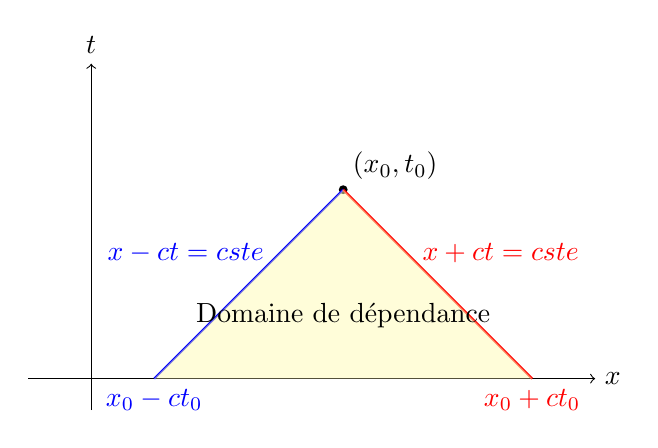
\begin{tikzpicture}[scale=0.8]
    \draw[->] (-1,0) -- (8,0) node[right] {$x$};
    \draw[->] (0,-0.5) -- (0,5) node[above] {$t$};
    % Point (x0, t0)
    \fill (4,3) circle (2pt) node[above right] {$(x_0, t_0)$};
    % Caractéristiques
    \draw[blue, thick] (4,3) -- (1,0) node[below] {$x_0-ct_0$};
    \draw[red, thick] (4,3) -- (7,0) node[below] {$x_0+ct_0$};
    % Domaine de dépendance
    \fill[yellow!30, opacity=0.5] (4,3) -- (1,0) -- (7,0) -- cycle;
    \node at (4, 1) {Domaine de d\'ependance};
    % Labels
    \node[blue] at (1.5, 2) {$x-ct=\text{cste}$};
    \node[red] at (6.5, 2) {$x+ct=\text{cste}$};
\end{tikzpicture}
\end{center}

\begin{formules}[title=\textbf{\'Equation des ondes 1D --- formules cl\'es}]
\begin{itemize}
    \item D'Alembert~: $u = \frac{1}{2}[g(x+ct)+g(x-ct)] + \frac{1}{2c}\int_{x-ct}^{x+ct} h(s)\, ds$.
    \item Caract\'eristiques~: $x \pm ct = \text{cste}$.
    \item Solution g\'en\'erale~: $u = F(x+ct) + G(x-ct)$.
\end{itemize}
\end{formules}

\subsection{Domaine de d\'ependance et d'influence}

\begin{definition}[Domaine de d\'ependance]
Le \textbf{domaine de d\'ependance} du point $(x_0, t_0)$ est le segment
$[x_0 - ct_0, x_0 + ct_0]$ de l'axe $t = 0$. La solution en $(x_0, t_0)$
ne d\'epend que des donn\'ees initiales sur ce segment.
\end{definition}

\begin{definition}[Domaine d'influence]
Le \textbf{domaine d'influence} du point $x_0$ sur l'axe $t = 0$ est
le c\^one $\{(x,t) : \abs{x - x_0} \leq ct,\; t > 0\}$.
\end{definition}

\begin{theoreme}[Vitesse finie de propagation]
Si les donn\'ees initiales $g$ et $h$ sont \`a support dans $[a,b]$,
alors $u(x,t) = 0$ pour $x \notin [a-ct, b+ct]$. L'information se
propage au plus \`a la vitesse $c$.
\end{theoreme}

\section{Conservation de l'\'energie}

\begin{theoreme}[Conservation de l'\'energie]
Si $u$ est solution de $u_{tt} = c^2\Delta u$ dans $\R^n$, l'\textbf{\'energie}~:
\begin{equation}\label{eq:energie_ondes}
    E(t) = \frac{1}{2}\int_{\R^n}
    \left(u_t^2 + c^2\abs{\nabla u}^2\right) dx
\end{equation}
est conserv\'ee~: $E(t) = E(0)$ pour tout $t \geq 0$.
\end{theoreme}

\begin{proof}
Calculons~:
\begin{align*}
    E'(t) &= \int_{\R^n} \left(u_t\, u_{tt} + c^2 \nabla u \cdot \nabla u_t\right) dx \\
    &= \int_{\R^n} u_t \left(u_{tt} - c^2\Delta u\right) dx = 0.
\end{align*}
La derni\`ere \'egalit\'e utilise l'int\'egration par parties
($\int \nabla u \cdot \nabla u_t = -\int u_t\, \Delta u$).
\end{proof}

\begin{corollaire}[Unicit\'e]
Le probl\`eme de Cauchy pour l'\'equation des ondes admet au plus une solution
(dans une classe de r\'egularit\'e ad\'equate).
\end{corollaire}

\section{Corde vibrante \`a extr\'emit\'es fixes}

\begin{exemple}
R\'esoudre~:
\[
    \begin{cases}
        u_{tt} = c^2 u_{xx}, & 0 < x < L,\; t > 0,\\
        u(0,t) = u(L,t) = 0,\\
        u(x,0) = g(x), \quad u_t(x,0) = h(x).
    \end{cases}
\]
Par s\'eparation des variables~:
\[
    u(x,t) = \sum_{n=1}^{\infty} \sin\!\left(\frac{n\pi x}{L}\right)
    \left[A_n \cos(\omega_n t) + B_n \sin(\omega_n t)\right],
\]
avec $\omega_n = \frac{cn\pi}{L}$ (fr\'equences propres). Les coefficients sont~:
\[
    A_n = \frac{2}{L}\int_0^L g(x)\sin\!\left(\frac{n\pi x}{L}\right) dx,
    \quad
    B_n = \frac{2}{L\omega_n}\int_0^L h(x)\sin\!\left(\frac{n\pi x}{L}\right) dx.
\]

La solution est une superposition de \textbf{modes propres} vibrant \`a des
fr\'equences $\omega_n = cn\pi/L$. La fr\'equence fondamentale est
$\omega_1 = c\pi/L$, les suivantes sont des \textbf{harmoniques}
$\omega_n = n\omega_1$.
\end{exemple}

\begin{intuition}
Chaque mode propre $\sin(n\pi x/L)\cos(\omega_n t)$ repr\'esente une
\textbf{onde stationnaire}~: la forme spatiale reste fixe, seule l'amplitude
oscille. La superposition de modes donne les formes complexes d'une corde
vibrante.
\end{intuition}

\section{\'Equation des ondes en dimension sup\'erieure}

\subsection{Dimension 3~: formule de Kirchhoff}

\begin{theoreme}[Formule de Kirchhoff]
La solution du probl\`eme de Cauchy en dimension 3~:
\[
    u_{tt} = c^2 \Delta u, \quad u(x,0) = g(x), \quad u_t(x,0) = h(x),
\]
est~:
\begin{equation}\label{eq:kirchhoff}
    u(x,t) = \frac{1}{4\pi c^2 t}\iint_{S(x,ct)} h(y)\, dS(y)
    + \frac{\partial}{\partial t}\left[\frac{1}{4\pi c^2 t}
    \iint_{S(x,ct)} g(y)\, dS(y)\right],
\end{equation}
o\`u $S(x,ct)$ est la sph\`ere de centre $x$ et de rayon $ct$.
\end{theoreme}

\begin{theoreme}[Principe de Huygens fort]
En dimension $n = 3$ (et plus g\'en\'eralement pour $n$ impair $\geq 3$),
le \textbf{principe de Huygens} est valide~: la solution en $(x,t)$ ne
d\'epend que des donn\'ees sur la sph\`ere $\abs{y-x} = ct$, pas dans
la boule. Physiquement, un signal ponctuel produit un front d'onde net
qui passe et s'\'eteint.
\end{theoreme}

\subsection{Dimension 2~: formule de Poisson}

\begin{theoreme}[Formule de Poisson --- dimension 2]
En dimension 2, la solution est~:
\begin{equation}\label{eq:poisson_ondes_2d}
    u(x,t) = \frac{1}{2\pi c}\iint_{B(x,ct)}
    \frac{h(y)}{\sqrt{c^2 t^2 - \abs{y-x}^2}}\, dy
    + \frac{\partial}{\partial t}\left[\frac{1}{2\pi c}\iint_{B(x,ct)}
    \frac{g(y)}{\sqrt{c^2 t^2 - \abs{y-x}^2}}\, dy\right].
\end{equation}
\end{theoreme}

\begin{attention}[title=\textbf{Pas de principe de Huygens en dimension paire}]
En dimension 2, la solution d\'epend des donn\'ees dans toute la boule
$B(x,ct)$, pas seulement sur le cercle. C'est pourquoi les ondes sur
l'eau laissent une tra\^in\'ee derri\`ere elles (contrairement aux ondes
sonores en 3D).
\end{attention}

\section{\'Equation des ondes avec dissipation}

L'\'equation des ondes amorties s'\'ecrit~:
\[
    u_{tt} + 2\gamma u_t = c^2 \Delta u, \quad \gamma > 0.
\]
Le terme $2\gamma u_t$ mod\'elise un frottement proportionnel \`a la vitesse.

\begin{proposition}[D\'ecroissance de l'\'energie]
Pour l'\'equation amortie, l'\'energie d\'ecro\^it~:
\[
    E'(t) = -2\gamma \int_{\R^n} u_t^2\, dx \leq 0.
\]
\end{proposition}

\section{Exercices}

\begin{exercice}
Utiliser la formule de d'Alembert pour r\'esoudre $u_{tt} = u_{xx}$ avec
$u(x,0) = e^{-x^2}$ et $u_t(x,0) = 0$. Tracer la solution pour $t = 0, 1, 2$.
\end{exercice}

\begin{exercice}
R\'esoudre $u_{tt} = 4u_{xx}$ avec $u(x,0) = 0$ et
$u_t(x,0) = \mathbf{1}_{[-1,1]}(x)$. D\'eterminer le domaine de
d\'ependance et tracer la solution.
\end{exercice}

\begin{exercice}
Corde vibrante~: r\'esoudre $u_{tt} = u_{xx}$ sur $(0,\pi)$ avec
$u(0,t) = u(\pi,t) = 0$, $u(x,0) = \sin(x)\sin(2x)$, $u_t(x,0) = 0$.
\end{exercice}

\begin{exercice}
Montrer que la conservation de l'\'energie implique l'unicit\'e pour
le probl\`eme de Cauchy.
\end{exercice}

\begin{exercice}[R\'eflexion sur un bord fixe]
Soit $u_{tt} = c^2 u_{xx}$ pour $x > 0$, $t > 0$ avec $u(0,t) = 0$ et
donn\'ees initiales \`a support compact dans $(0,\infty)$. Utiliser la
m\'ethode des images (prolongement impair) pour construire la solution.
\end{exercice}

\begin{exercice}
Pour l'\'equation des ondes amorties $u_{tt} + 2\gamma u_t = c^2 u_{xx}$,
montrer que l'\'energie $E(t) \leq E(0)\, e^{-2\gamma t}$.
\end{exercice}

\begin{exercice}
V\'erifier la formule de Kirchhoff en 3D pour le cas $g = 0$,
$h(x) = 1$ (donn\'ee constante). Trouver explicitement $u(0,t)$.
\end{exercice}

\begin{exercice}[Principe de Duhamel pour les ondes]
Montrer que la solution de $u_{tt} - c^2 u_{xx} = f(x,t)$ avec
$u(x,0) = u_t(x,0) = 0$ est~:
\[
    u(x,t) = \frac{1}{2c}\int_0^t \int_{x-c(t-s)}^{x+c(t-s)} f(y,s)\, dy\, ds.
\]
\end{exercice}
